\documentclass[a4paper,11pt,eval]{nsi} % COMPILE WITH DRAFT
\usepackage{hyperref}

\pagestyle{empty}
\begin{document}

\textcolor{UGLiBlue}{Jeudi 13/03/2025}\\
\classe{\premiere spe}
\titre{\includegraphics[width=3cm]{CAN.png} Interro 1}
\maketitle

\begin{enumerate}[itemsep=1em]
	\item $9 \times 0{,}4=$  $\ldots$
	\item $3-\dfrac{2}{3}= $ $\ldots$
	\item Donner l'écriture décimale de :  $5\times10^2+5+6\times 10^{-1}$.
	\item Résoudre l'équation $3x+6=0$.
	\item $4$ croissants coûtent  $3{,}60$ €.  Combien coûtent $2$ croissants ?
                        
	\item Calculer la fréquence de boules noires parmi ces boules :\\
          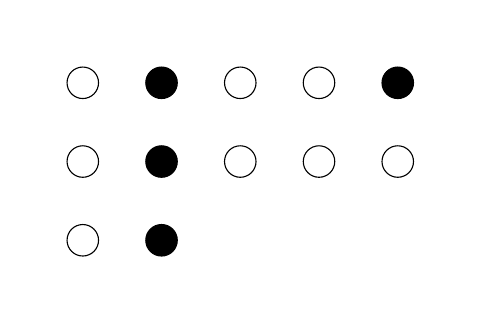
\begin{tikzpicture}[baseline]

    \tikzset{
      point/.style={
        thick,
        draw,
        cross out,
        inner sep=0pt,
        minimum width=5pt,
        minimum height=5pt,
      },
    }
    \clip (-0.7,-2.7) rectangle (4.7,0.7);
    	
	 \filldraw[color={black},fill={white}] (0,0) circle (0.2);
	
	 \filldraw[color={black},fill={black}] (1,0) circle (0.2);
	
	 \filldraw[color={black},fill={white}] (2,0) circle (0.2);
	
	 \filldraw[color={black},fill={white}] (3,0) circle (0.2);
	
	 \filldraw[color={black},fill={black}] (4,0) circle (0.2);
	
	 \filldraw[color={black},fill={white}] (0,-1) circle (0.2);
	
	 \filldraw[color={black},fill={black}] (1,-1) circle (0.2);
	
	 \filldraw[color={black},fill={white}] (2,-1) circle (0.2);
	
	 \filldraw[color={black},fill={white}] (3,-1) circle (0.2);
	
	 \filldraw[color={black},fill={white}] (4,-1) circle (0.2);
	
	 \filldraw[color={black},fill={white}] (0,-2) circle (0.2);
	
	 \filldraw[color={black},fill={black}] (1,-2) circle (0.2);

\end{tikzpicture}\\
	\item Calculer l'expression  $x^2+5x+6$ pour $x=-2$.
	\item Calculer la moyenne de :
            $2\,\,\,; \,\,\,4\,\,\,; \,\,\,28\,\,\,; \,\,\,26$.
	\item $90$ $\%$ de $90= $ $\ldots$
	\item  $12{,}2$ L $=$ $\ldots$ m$^3$
\end{enumerate}

\newpage

\textcolor{UGLiBlue}{
\begin{enumerate}[itemsep=1em]
    \item $9 \times 0{,}4=9\times 4\times 0,1=3{,}6$
    \item $3-\dfrac{2}{3}= \dfrac{9}{3}-\dfrac{2}{3}=\dfrac{7}{3}$
    \item $5\times10^2+5+6\times 10^{-1}=500+5+0{,}5=505{,}6$
    \item On se ramène à une équation du type $a\times x=b$ :\\
              $\begin{aligned}
              3x+6&=0\\
             3x&=-6\\
                                  x&=\dfrac{-6}{3}=-\dfrac{2{\color[HTML]{2563a5}\boldsymbol{\times3}} }{1{\color[HTML]{2563a5}\boldsymbol{\times3}}}=-2
             \end{aligned}$\\
              L'équation $3x+6=0$ a pour solution $x=-2$.
    \item $4$ croissants coûtent  $3{,}60$ €, donc
                           $2$ croissants coûtent $2$ fois moins, soit : \\
                           $3{,}60\div 2=1{,}80$ €.
    \item La fréquence est donnée par le quotient : $\dfrac{\text{Nombre de boules noires}}{\text{Nombre total de boules}}=\dfrac{4}{12}=\dfrac{1{\color[HTML]{2563a5}\boldsymbol{\times4}} }{3{\color[HTML]{2563a5}\boldsymbol{\times4}}}=\dfrac{1}{3}$.
    \item 
                Pour $x=-2$, on obtient : $x^2+5x+6=(-2)^2+5\times (-2)+6=0$.  
    \item La moyenne est donnée par : $\dfrac{2+4+28+26}{4}=\dfrac{60}{4}=15$.
    \item           Prendre $90$ $\%$  de $90$ revient à prendre $9\times 10$ $\%$  de $90$.\\
                Comme $10$ $\%$  de $90$ vaut $9$ (pour prendre $10$ $\%$  d'une quantité, on la divise par $10$), alors
                $90$ $\%$ de $90=9\times 9=81$.       
    \item Comme $1$ L= $0,001$ m$^3$, $12{,}2$ L $=0{,}012\,2$  m$^3$.
\end{enumerate}
}
\end{document}